\section{Discussion} % (fold)
\label{sec:discussion}
In this section we will look back at the problem introduced in section \ref{sec:introduction} and evaluate the implementation of Raft. This will be done by comparing our test results with the requirements stated in section \ref{sec:requirements}. Doing this, we can reflect on the overall goal of the project i.e. to gain deeper knowledge of Raft. Further extensions and improvements to the end product will then be proposed and discussed.

\subsection{Requirements evaluation}
The requirements stated that we should have tool that illustrated a given distributed system with a number of servers, implementing Raft as a solution to finding consensus in the presence of faulty servers. We evaluate each functional requirement by referring to the results in section~\ref{sec:results} as following:

\begin{enumerate}
\item The tool indeed illustrates a distributed system where the user can issue commands both related to Raft but also for simulation purposes.
\item The tool provides fault tolerance by utilising Raft, in the since that it will tolerate servers that crash in a non-Byzantine manner.
\item The user can give parameters for: time between heartbeats, how many servers the system should consist of, latency for RPC's, and interval for random election timers.
\item The user can crash a server through the client by issuing the correct command for it in the console.
    \begin{enumerate}
    \item The implementation of Raft ensures that a new leader is elected, once a candidate achieves a majority vote.
    \end{enumerate}
\item The user can request that an entry is replicated through the system by issuing the correct command for it in the console.
\item The tool visualized the system through a console GUI.
\end{enumerate}
\\
It is hard to verify whether we have met the quality requirement or not. These it due to the lag of static behaviour of the system caused by the the randomized election time outs and general concurrent aspects of the system. This is discussed in further detail in the next section.

\subsection{Reflection on goal}
The goal of this project was to learn about what is the state of the art in terms of solving the consensus problem. In order to do this, our approach was to gain knowledge about Raft through implementing it in a simulated environment.
The requirements for the implementation stated that it should provide a tool for visualising the behaviour of Raft. \\
We divided our tests into white- and black box tests in order to document our development process better by testing the behaviour in the white box tests and come with example tests when verifying the solution itself in the black box tests. But the black box tests do not verify the correctness of the implementation, since they do not cover to whole space of possible scenarios. Another way to verify our implementation would have been to use a formal verification tool such as SPIN, which is used for testing models of concurrent systems. But this would require us to develop a whole new solution in another language i.e. Promela which conflicts with our main goal, which was to utilize the flexibility and small over head provided by Javascript.

In terms of the correctness of the implementation of Raft, referring back to the properties for non-Byzantine failure tolerant systems listed in section~\ref{sec:introduction}, the choice of platform again provides a poor basis for a formal verification. But it can be argued that by adopting the behaviour specified in the Raft paper thus also the safety properties, that our implementation upholds the properties of validity and integrity in the cases we have chosen to test.

\subsection{Experiences}

The biggest challenge of implementing the Raft algorithm is to implement and test the situations in parallel (such as mentioned with log replication and RPC's in elections) and the leader election driven by a randomly initialized timer.

In the situations in parallel we have suggested the method of using a protocol supporting both direct and delayed communicating between servers in section~\ref{sub:requestvote_rpc}. This made it easy to test the behaviour involving RPC's, but there are challenges in parallel computing that cannot be hidden with abstractions. The first one is race conditions which we experienced in the simulation when the RPC delay is to high in relation to the heartbeat interval. If the leader e.g. replicates a log entry $x\rightarrow5$ to a follower and before the follower is able to respond to the RPC (e.g. because of latency) a new hearbeat interval is started and the leader blindly tries to replicate the same log entry with $x\rightarrow5$. This will make the follower append the same entry twice. The situation is illustrated in figure~\ref{fig:replication_race_condition}. Although we discovered this implementation issue it did not ruin the consensus due to the safety rules of Raft and the problem was fixed by making the log appending method of followers idempotent as described in section~\ref{sub:log_replication_implementation}, but it illustrates that the solution of abstracting away parallel operations does not solve the problem of testing fully.

\begin{figure}
\centering
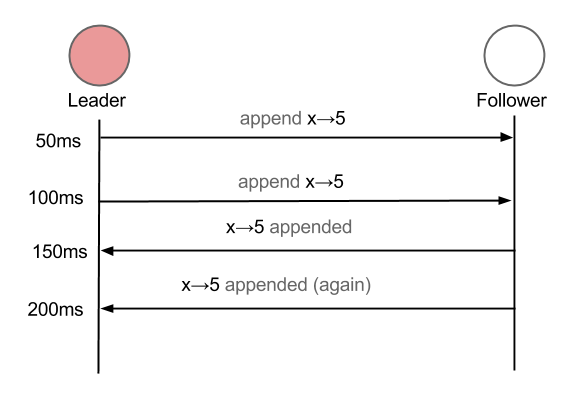
\includegraphics[scale = 0.4]{figures/replication_race_condition.png}
\caption{A situation with possible race condition when idempotent log appends is not implemented. This figure illustrates that some situations are only present when in parallel (or asynchronous).}
\label{fig:replication_race_condition}
\end{figure}

The random election timer used in leader election in Raft as explained in section~\ref{sub:requestvote_rpc} made it hard to test the leader election. The solution for white box tests was to invoke methods to simulate the random timer. To test the leader election with the random timer we used a delay as explained in section~\ref{subsub:evaluation_test_tests}. One problem with tests as these is that if the tests fail in a given situation is is impossible to replicate the random situation. Another problem is that if the system testing relies on faults in random situation it is not a system you should trust. The last problem is that slow tests slow down the development flow such that every test will be a tradeof of much slower test suites.

\subsection{Future work}

The code for this project is open source and can easily be extended. One interesting extension would be to visualize the server in a graph with visualized RPC-requests to see the communication between the servers and maybe the data send back and foward.

As mentioned it is hard to verify a Raft implementation because some parts of algorithm rely on parallelism, random values and timing. A future project could be about how such components can be verified either formally or by using tests.

A third extension for further work would be to build or use a monitoring tool to measure the availability of the implementation. The simulation tools build in this project could then be exposed to relaistic loads and operations in a longer period of time in which the monitoring tool could measure and an estimated a Mean time between failures to calculate the availability and easier verify the Timing independence quality requirement specified in section~\ref{sec:requirements}.

% Using random election timeout and trouble with testing.

% section discussion (end)
